% Definindo o tipo de documento
\documentclass[letterpaper]{article}

\usepackage[latin1]{inputenc}
\usepackage[brazil]{babel}
\usepackage{indentfirst}
\usepackage{fancyhdr}
\usepackage[noprefix]{nomencl}
\usepackage[letterpaper,
            ps2pdf,
            pdfborder={0 0 0},
            colorlinks={false},
            pdfpagemode={None},
            pdftitle={},
            pdfauthor={Victor de Abreu Iizuka et al},
            pdfsubject={Relaxacao Lagrangeana},
            pdfkeywords={Relaxacao Lagrangeana },
            pdfview={FitBH}]{hyperref}
\usepackage[T1]{fontenc}
\usepackage[dvips]{graphicx}
\usepackage[algoruled,portugues,linesnumbered]{algorithm2e}
\usepackage{amsmath}
\usepackage{amsfonts}

\pagestyle{fancy}
\addtolength{\headheight}{2pt}
\fancyhead{}
\fancyhead[L]{\large{\textsf{Victor de A. I.}}}
\fancyhead[R]{\textsl{\leftmark}}
\fancyfoot{}
\fancyfoot[R]{\small{\textsl{p�g. \thepage{} de \pageref{fimdoc}}}}
\fancyfoot[C]{\small{\textsf{Relaxa��o Lagrangeana}}}
\fancyfoot[L]{\small{\textsl{\today}}}
\renewcommand{\footrulewidth}{0.4pt}

\newcommand{\aspas}[1]{``#1''}
\newcommand{\estr}[1]{\textsl{\foreignlanguage{american}{#1}}}
\newcommand{\thead}[1]{\textbf{#1}}
\newcommand{\sigla}[1]{\texttt{#1}}
\newcommand{\converter}[2]{\small\textsl{#1 $\pm{}$ #2}\normalsize}
\newcommand{\pcmcrc}{Problema do Caminho mais Curto com Restri��o de Custo}
\newcommand{\spcmcrc}{PCMCRC}
\newcommand{\mpcmcrc}{problema do caminho mais curto com restri��o de custo}
\newcommand{\cmcrc}{caminho mais curto com restri��o de custo}
\newcommand{\pcmc}{Problema do Caminho mais Curto}
\newcommand{\mpcmc}{problema do caminho mais curto}
\newcommand{\cmc}{caminho mais curto}
\newcommand{\knap}{Mochila Bin�ria}
\newcommand{\mknap}{mochila bin�ria}
\newcommand{\rellag}{relaxa��o lagrangeana}
\newcommand{\rl}[1]{\textit{RL#1}}

\hyphenation{a-de-q�a-dos a-li-nha-dos a-li-nha-men-to a-li-nha-men-tos a-lign-ments a-tra-v�s BAliBASE e-xem-plo ge-ne-ra-li-za-da glo-bal-men-te  pu-bli-ca-das re-fe-r�n-cia re-pe-ti-��es se-me-lhan-�a UPGMA vi-zi-nhas si-na-li-za-das in-ter-ca-la-dos res-tri-��es pro-ble-ma res-tri-��o}


% T�tulo e autor
\title{Relaxa��o Lagrangeana: \\ \pcmcrc}
\author{Victor de Abreu Iizuka}

% Come�ando o documento
\begin{document}

% Imprimindo o t�tulo
\maketitle{}
% Imprimindo o �ndice
\tableofcontents{}
\listoftables{}
\listoffigures{}
%\listofalgorithms{}

\thispagestyle{empty}
\newpage

\section{Introdu��o}
\label{sec:intro}
Dado um grafo simples n�o-orientado \textit{G = (V,E)} tal que, a cada aresta $e \in E$ 
est� associado um custo positivo $c_{e}$ e uma dist�ncia $d_{e}$. Seja $P$ um caminho em $G$,
o custo de $P$ � dado como $c(P) = \sum_{e \in P} c_{e}$ e o comprimento de $P$ � dado como
$d(P) = \sum_{e \in P} d_{e}$.

Dado um inteiro positivo $C$, e dois v�rtices distintos $s$ e $t$, o \pcmcrc{} (\textit{\spcmcrc{}}), 
para o grafo $G$, � encontrar o menor caminho $P^{*}$ que liga os v�rtices $s$ e $t$ em $G$ 
tal que $c(P^{*}) \le C$.


\section{Objetivo}
\label{sec:objetivo}

O objetivo deste trabalho foi implementar um algoritmo que use relaxa��o lagrangeana
para encontrar o \cmcrc{} usando a linguagem C.


\section{Formula��o PLI para o Problema}
\label{sec:form_pcmcrc}

A formula��o do \pcmcrc{} � a mesma formula��o do \pcmc{} adicionando a restri��o de custo $c(P^{*}) \le C$.
Ent�o temos o seguinte modelo para o \mpcmcrc{}: \\

Fun��o Objetivo:

\begin{equation}
\label{eq:fo_pli}
z = \min \sum_{(i, j) \in E} d_{i, j} \cdot x_{i, j}
\end{equation} \\

Sujeito a:

\begin{align}
\label{eq:restr_pli_pcmc1}
&\sum_{j \in V} x_{s, j} = 1 \\
\label{eq:restr_pli_pcmc2}
&\sum_{i \in V} x_{i, t} = 1 \\
\label{eq:restr_pli_pcmc3}
&\sum_{j \in V} x_{i, j} - \sum_{j \in V} x_{j, i} = 0, \qquad \forall i \in V\backslash\{s, t\}
\end{align}

\begin{equation}
\label{eq:restr_pli_knap}
\sum_{(i, j) \in E} c_{i, j} . x_{i, j} \le C
\end{equation}

\begin{equation}
\label{eq:restr_pli_x}
x_{i, j} \in \mathbb{B}, \qquad \forall (i, j) \in E
\end{equation} \\

Onde: 

\begin{itemize}
\item{$d_{i, j}$: Dist�ncia do v�rtice $i$ para o v�rtice $j$.}
\item{$c_{i, j}$: Custo do v�rtice $i$ para o v�rtice $j$.}
\item{$x_{i, j}$: 1 se a aresta ($i$, $j$) pertence ao caminho e 0 caso contr�rio.}
\item{$s$: V�rtice origem.}
\item{$t$: V�rtice destino.}
\end{itemize}

Observe que as restri��es (\ref{eq:restr_pli_pcmc1}), (\ref{eq:restr_pli_pcmc2}) e (\ref{eq:restr_pli_pcmc3}) 
s�o o conjunto de restri��es do problema cl�ssico do \cmc{}, onde:

\begin{itemize}
\item{Restri��o (\ref{eq:restr_pli_pcmc1}): S� � permitida uma aresta saindo do v�rtice origem $s$.}
\item{Restri��o (\ref{eq:restr_pli_pcmc2}): S� � permitida uma aresta entrando no v�rtice destino $t$.}
\item{Restri��o (\ref{eq:restr_pli_pcmc3}): Um v�rtice $i \in V\backslash\{s, t\}$ no caminho deve possuir apenas 
uma aresta entrando e uma aresta saindo.}
\end{itemize}

A restri��o (\ref{eq:restr_pli_knap}) � a restri��o do tipo \knap{} que representa a restri��o de custo.

\section{Limitante Primal}
\label{sec:limprim}

O Limitante Primal (Limitante Superior) para o \pcmcrc{} � encontrado fazendo os seguintes passos:

\begin{enumerate}
\item{$l \leftarrow 1$.}
\item{Seja $d[i][j]$ o valor da dist�ncia da aresta $(i, j)$ e $c[i][j]$ o valor do custo da aresta $(i, j)$.}
\item{Enquanto $l \ge 0$, Executar o shortest\_path()~(\ref{alg:shortest_path}), 
usando como dist�ncia $l \cdot d[i][j] + (1 - l) \cdot c[i][j]$ para todas as arestas $(i, j) \in E$}
\item{Verificar se a restri��o de custo � satisfeita. Se for satisfeita v� para o passo 6.}
\item{Sen�o $l \leftarrow l - \xi$ onde $ 0 < \xi < 1$ e volte para passo 3.}
\item{Calcular o valor da solu��o encontrada.}
\end{enumerate}

No melhor dos casos o limitante primal vai ser o valor da solu��o �tima do \mpcmcrc{}. Quando $l = 0$ o problema
vai minimizar o caminho usando os custos como dist�ncia, se este caminho respeita a restri��o de custo,
esta solu��o ir� ser vi�vel.


\section{Relaxa��o Lagrangeana}
\label{sec:relaxlag}

A relaxa��o lagrangeana foi realizada sobre dois conjuntos de restri��es. A Relaxa��o onde
o conjunto de restri��es do \cmc{} foram dualizadas � chamada de \rl{1}. A Relaxa��o 
onde a restri��o do tipo \knap{} foi dualizada � chamada de \rl{2}.

O Problema Primal Lagrangeano para cada relaxa��o � diferente. Para a relaxa��o \rl{1}, o problema
primal lagrangeano � o Problema da \knap{}. J� para a relaxa��o \rl{2}, o problema primal lagrangeano � o \pcmc{}.

\subsection{\rl{1} - Problema da \knap{}}
\label{subsec:relaxlag_rl1}

A relaxa��o \rl{1} tem como problema primal lagrangeano o Problema da \knap{}. Este � um problema de 
maximiza��o onde desejamos pegar o maior n�mero de \aspas{itens} satisfazendo a restri��o de peso da mochila. 
Temos que $\min z = max -z$, ent�o transformaremos o problema de minimiza��o para um 
de maximiza��o.

Logo temos o seguinte modelo para o problema primal lagrangeano da relaxa��o \rl{1}: \\

Fun��o Objetivo:

\begin{align}
\label{eq:fo_rl1}
z(u) = \max -(&\sum_{j \in V} ((d_{s, j} + u_{s}) \cdot x_{s, j}) + \nonumber\\
&\sum_{i \in V} ((d_{i, t} + u_{t}) \cdot x_{i, t}) + \\
&\sum_{j \in V\backslash\{s, t\}} \sum_{i \in V} (d_{i, j} \cdot x_{i, j}) - u_{s} - u_{t}) \nonumber
\end{align} \\

Sujeito a:

\begin{equation}
\label{eq:restr_rl1_knap}
\sum_{(i, j) \in E} c_{i, j} . x_{i, j} \le C
\end{equation}

\begin{equation}
\label{eq:restr_rl1_x}
x_{i, j} \in \mathbb{B}, \qquad \forall (i, j) \in E
\end{equation} \\

\subsubsection{Custos Lagrangeanos}
\label{subsubsec:custo_lag_rl1}

Para a relaxa��o \rl{1}, os custos lagrangeanos s�o os custos relacionados ao v�rtice origem $s$ e 
ao v�rtice destino $t$. Como o grafo � simples e n�o-orientado temos que $x_{i, j} = x_{j, i}$, logo 
os multiplicadores associados a restri��o (\ref{eq:restr_pli_pcmc3}) do problema original se anulam.
Ent�o temos os seguintes custos lagrangeanos:

\begin{align}
\tilde{c}_{s, j} = d_{s, j} + u_{s}, \qquad &\text{para o v�rtice s}. \nonumber\\
\tilde{c}_{i, t} = d_{i, t} + u_{t}, \qquad &\text{para o v�rtice t}. \nonumber\\
\tilde{c}_{i, j} = d_{i, j}, \qquad &\text{para os v�rtices diferentes de s e t}. \nonumber
\end{align}

\subsubsection{Algoritmo}
\label{subsubsec:alg_rl1}

O algoritmo implementado para resolver o Problema da \knap{} � um algoritmo pseudo-polinomial com 
complexidade de tempo de $O(C \cdot |E|)$ TODO .

%fazer algoritmo

\subsection{\rl{2} - \pcmc{}}
\label{subsec:relaxlag_rl2}

A relaxa��o \rl{2} tem como problema primal lagrangeano o \pcmc{}. Dado um grafo $G = (V, E)$ simples 
n�o-orientado e dois v�rtices distintos $s$ e $t$, o \mpcmc{} � encontrar o menor caminho $P^{*}$ que 
liga os v�rtices $s$ e $t$.

O problema primal lagrangeano da relaxa��o \rl{2} possui o seguinte modelo:

Fun��o Objetivo:

\begin{equation}
\label{eq:fo_rl2}
z(u) = \min \sum_{(i, j) \in E} (d_{i, j} + u \cdot c_{i, j}). x_{i, j} - u \cdot C
\end{equation} \\

Sujeito a:

\begin{align}
\label{eq:restr_rl2_pcmc}
&\sum_{j \in V} x_{s, j} = 1 \nonumber \\
&\sum_{i \in V} x_{i, t} = 1 \\
&\sum_{j \in V} x_{i, j} - \sum_{j \in V} x_{j, i} = 1, \qquad \forall i \in V\backslash\{s, t\} \nonumber
\end{align}

\begin{equation}
\label{eq:restr_rl2_x}
x_{i, j} \in \mathbb{B}, \qquad \forall (i, j) \in E
\end{equation} \\

\subsubsection{Custos Lagrangeanos}
\label{subsubsec:custo_lag_rl2}

Para a relaxa��o \rl{2}, o custo lagrangeano � o custo relacionado a restri��o de custo 
do caminho (\ref{eq:restr_pli_knap}).

\begin{align}
\tilde{c}_{i, j} = d_{i, j} + u \cdot c_{i, j}. \nonumber\\
\end{align}

\subsubsection{Algoritmo}
\label{subsubsec:alg_rl1}

O algoritmo implementado para resolver o \pcmc{} � o algoritmo de Dijkstra que possui 
complexidade de tempo de $O(|V|^{2})$ TODO .

% fazer algoritmo

\subsection{For�a dos Limitantes}
\label{subsec:str_bound}



\section{An�lise dos Resultados}
\label{sec:an_res}

\subsection{Caracter�sticas da M�quina}
\label{subsec:car_maq}

\begin{itemize}
\item{Processador: Intel(R) Core(TM)2 Duo T8100 @ 2.10 GHz}
\item{Mem�ria RAM: 4 GB}
\end{itemize}

\subsection{Par�metros de Entrada}
\label{subsec:par_ent}

O programa recebe como par�metros de entrada a relaxa��o escolhida, o arquivo da inst�ncia a ser testada 
e o arquivo contendo os par�metros usados no m�todo do subgradiente.

Para o m�todo do subgradiente foram usados os seguintes par�metros: fator multiplicativo de $u_{k}$($\alpha$), 
n�mero m�ximo de itera��es do m�todo do subgradiente(MAX\_ITER) e n�mero de itera��es necess�rias para
alterar o valor de $\alpha$ caso o limitante dual n�o seja modificado (MAX\_ITER\_NO\_IMPROV).

\begin{table}[htb]
\centering
\sffamily
\begin{tabular}{c|c|c|c}
\thead{par�metro$\backslash$arquivo} & \thead{param1} & \thead{param2} & \thead{param3} \\
\hline{}
$\alpha$ & 2 & 0.1 & 0.01 \\
\text{MAX\_ITER} & 600 & 1000 & 800 \\
\text{MAX\_ITER\_NO\_IMPROV} & 10 & 5 & 15  
\end{tabular}
\label{tab:par_subgrad}
\caption{Par�metros usados na execu��o do programa para ambas relaxa��es.}
\normalfont
\end{table}

\subsection{Coment�rios}
\label{subsec:coment}

Podemos observar alguns pontos ao executar o algoritmo:

\begin{itemize}
\item{A relaxa��o \rl{1} obteve limitantes duais ru�ns em rela��o aos obtidos pela relaxa��o \rl{2}. Isto 
ocorre devido ao fato que, na maioria das vezes, o resultado da mochila n�o � um caminho, logo a solu��o 
da relaxa��o n�o � vi�vel para o \pcmcrc, desta forma n�o gera bons limitantes primais. Outro fator que pode
ter influenciado � o for�a do limitante gerado pela relaxa��o \rl{2}, que � mais forte em rela��o ao da
relaxa��o \rl{1}.}
\item{Em geral, o tempo total usado pela relaxa��o \rl{2} � menor em rela��o ao obtido pela relaxa��o \rl{1}.}
\item{Se reduzimos o valor de $\alpha$, o m�todo do subgradiente executa mais itera��es para encontrar um
bom limitante dual.}
\item{Se o valor de MAX\_ITER\_NO\_IMPROV for alto, o limitante dual pode n�o sofrer altera��es, mas se for baixo
o valor de $\alpha$ pode ser reduzido com mais frequ�ncia.}
\end{itemize}

\section{Conclus�o}
\label{sec:conclusao}
A \rellag{} � uma boa ferramenta para encontrarmos solu��es vi�veis sabendo a qualidade da solu��o 
para problemas computacionalmente dif�ceis\footnote{Problemas das classes NP, Np-dif�cil e NP-completo}. 

Dependendo da restri��o que escolhemos dualizar, o limitante gerado pelo problema relaxado pode ser ru�m, 
dificultando a converg�ncia do m�todo do subgradiente.

Os resultados poderiam ser melhorados caso a \rellag{} seja usada em conjunto com outro m�todo, de \textit{branch-and-bound}, por exemplo.


\appendix
\section{Ap�ndice}
%\subsection{Algoritmos Implementados}
\label{appsec:alg}

Nesta se��o se encontra os algoritmos usados na implementa��o do trabalho.

\begin{algorithm}[!ht]
\caption{knapsack\_dp($G = (V, E)$, $d$, $w$, $W$)}
\Entrada{Grafo $G$ simples n�o-orientado, $d$ dist�ncias das arestas de $G$, 
$w$ custos das arestas de $G$ e $W$ peso m�ximo da mochila.}
\Saida{Custo dos itens escolhidos e matriz de programa��o din�mica preenchida.}
\BlankLine
\tcc{Inicializa��o}
\Para{$j = 0$ \Ate $W + 1$}{
	M[0][j] $\leftarrow$ $0$\;
}
\Para{$i = 0$ \Ate $|E| + 1$}{
	M[i][0] $\leftarrow$ $0$\;
}
\BlankLine
\Para{$i = 1$ \Ate $|E| + 1$}{ 
	\Para{$j = 1$ \Ate $W + 1$}{
		\uSe{$w_{i} \le j$}{
			\uSe{$d_{i} + M[i - 1][j - w_{i}] > M[i][j]$}{
				$M[i][j] \leftarrow d_{i} + M[i - 1][j - w_{i}]$\;
			}
			\Senao{
				$M[i][j] \leftarrow M[i - 1][j]$\;
			}
		}
		\Senao{
			$M[i][j] \leftarrow M[i - 1][j]$\;
		}
	}
}
\Retorna{($M[|E|, W], M$)}
\label{alg:knap_dp}
\end{algorithm}

\begin{algorithm}[!ht]
\caption{knapsack\_sol($d$, $w$, $m$, $W$, $M$, $X$)}
\Entrada{$w$ custos das arestas de $G$, 
$m$ n�mero de arestas, $W$ peso m�ximo da mochila, $M$ matriz de
programa��o din�mica preenchida}
\Saida{Conjunto solu��o.}
\BlankLine
\Se{$m \neq 0$}{
	\uSe{$M[m][W] = M[m - 1][W]$}{
		$knapsack\_sol(d, w, m - 1, W, M, X)$\;
	}
	\Senao{
		$X \leftarrow X \cup \{m\}$\;
		$knapsack\_sol(d, w, m - 1, W - w_{m}, M, X)$\;
	}
}
\BlankLine
\label{alg:knap_sol}
\end{algorithm}

\begin{algorithm}[!ht]
\caption{knapsack($G = (V, E)$, $d$, $w$, $W$)}
\Entrada{Grafo $G$ simples n�o-orientado, $d$ dist�ncias das arestas de $G$, 
$w$ custos das arestas de $G$ e $W$ peso m�ximo da mochila.}
\Saida{Custo dos itens escolhidos e conjunto solu��o.}
\BlankLine
\tcc{Inicializa��o}
$X \leftarrow \emptyset$\;
\BlankLine
$(cost, M) \leftarrow knapsack\_dp(G, d, w, W)$\;
\BlankLine
$knapsack\_sol(w, |E|, W, M, X)$\;
\Retorna{($cost, X$)}
\label{alg:knap}
\end{algorithm}

\begin{algorithm}[!ht]
\caption{Dijkstra($G = (V, E)$, $w$, $s$, $t$)}
\Entrada{Grafo $G$ simples n�o-orientado, $w$ dist�ncias das arestas de $G$ e dois v�rtices distintos $s$ e $t$.}
\Saida{Vetor com os valores das dist�ncias e vetor com os valores de predecessores.}
\BlankLine
\tcc{Inicializa��o}
\ParaCada{v�rtice $v \in V$}{
	dist[v] $\leftarrow$ $\infty$\;
	pred[v] $\leftarrow$ -1\;
}
dist[0] $\leftarrow$ 0\;
\BlankLine
\tcc{Conjunto de v�rtices onde as dist�ncias j� foram determinadas}
$S$ $\leftarrow$ $\emptyset$\;
\tcc{Conjunto dos v�rtices n�o analisados}
$Q$ $\leftarrow$ $V$\;
\BlankLine
\Enqto{$Q$ $\neq$ $\emptyset$}{ 
	$u$ $\leftarrow$ EXTRACT\_MIN($Q$)\;
	$S$ $\leftarrow$ $S$ $\cup$ \{$u$\}\;
	\ParaCada{v�rtice $v \in$ ADJ($u$)}{
		\Se{dist[u] + $w[u][v]$ < dist[v]}{
			dist[v] $\leftarrow$ dist[u] + $w[u][v]$\;
			pred[v] $\leftarrow$ $u$\;
		}
	}
}
\Retorna{($dist, pred$)}

\label{alg:dijkstra}
\end{algorithm}

\begin{algorithm}[!ht]
\caption{shortest\_path($G = (V, E)$, $w$, $s$, $t$)}
\Entrada{Grafo $G$ simples n�o-orientado, $w$ dist�ncias das arestas de $G$ e dois v�rtices distintos $s$ e $t$.}
\Saida{Custo do caminho e as arestas pertencentes ao caminho.}
\BlankLine
\tcc{Inicializa��o}
$X \leftarrow \emptyset$\;
$(dist, pred) \leftarrow Dijkstra(G, w, s, t)$\;
\BlankLine
$i \leftarrow t$\;
\Enqto{$i \neq s$}{
	$j \leftarrow pred[i]$\;
	$X \leftarrow X \cup \{(i, j)\}$\;
	$i \leftarrow j$\;
}
\BlankLine
\Retorna{($dist[t], X$)}

\label{alg:shortest_path}
\end{algorithm}


\subsection{Tabelas}
\label{appsec:tables}

\begin{table}[htb]
\centering
\sffamily
  \begin{tabular}{c|c|c|c|c}
  \thead{Inst�ncia} & \thead{lim. superior} & \thead{tempo lim.sup.} & \thead{lim.inferior} & \thead{tempo lim.inf.} \\
  \hline{}
	v100\_d10 & $ 144.000000$ &  810 microseg  & $ 346.000000$ &  3360 microseg \\
	v100\_d20 & $ 154.000000$ &  3068 microseg  & $ 216.000000$ &  5167 microseg \\
	v100\_d30 & $ 142.000000$ &  900 microseg  & $ 305.000000$ &  6802 microseg \\
	v100\_d40 & $ 145.000000$ &  3978 microseg  & $ 164.000000$ &  6489 microseg \\
	v100\_d5 & $ 244.000000$ &  11672 microseg  & $ 310.000000$ &  2848 microseg \\
	v10\_d50 & $ 200.000000$ &  222 microseg  & $ 324.000000$ &  249 microseg \\
	v10\_d60 & $ 142.000000$ &  65 microseg  & $ 143.000000$ &  186 microseg \\
	v10\_d70 & $ 171.000000$ &  238 microseg  & $ 175.000000$ &  226 microseg \\
	v10\_d80 & $ 162.000000$ &  222 microseg  & $ 294.000000$ &  194 microseg \\
	v30\_d30 & $ 160.000000$ &  541 microseg  & $ 220.000000$ &  552 microseg \\
	v30\_d40 & $ 188.000000$ &  1991 microseg  & $ 346.000000$ &  813 microseg \\
	v30\_d50 & $ 143.000000$ &  163 microseg  & $ 154.000000$ &  1644 microseg \\
	v30\_d60 & $ 148.000000$ &  1371 microseg  & $ 333.000000$ &  880 microseg \\
	v30\_d70 & $ 145.000000$ &  436 microseg  & $ 203.000000$ &  995 microseg \\
	v40\_d20 & $ 213.000000$ &  5173 microseg  & $ 221.000000$ &  845 microseg \\
	v40\_d30 & $ 143.000000$ &  155 microseg  & $ 285.000000$ &  1588 microseg \\
	v40\_d40 & $ 155.000000$ &  1434 microseg  & $ 290.000000$ &  1036 microseg \\
	v40\_d50 & $ 150.000000$ &  2986 microseg  & $ 307.000000$ &  1306 microseg \\
	v40\_d60 & $ 178.000000$ &  3708 microseg  & $ 180.000000$ &  2538 microseg \\
	v60\_d10 & $ 253.000000$ &  1706 microseg  & $ 330.000000$ &  1582 microseg \\
	v60\_d20 & $ 271.000000$ &  9232 microseg  & $ 300.000000$ &  3988 microseg \\
	v60\_d30 & $ 177.000000$ &  6774 microseg  & $ 213.000000$ &  3596 microseg \\
	v60\_d40 & $ 362.000000$ &  12803 microseg  & $ 407.000000$ &  7835 microseg \\
	v60\_d50 & $ 161.000000$ &  8150 microseg  & $ 332.000000$ &  3076 microseg \\
  \end{tabular}
  \caption[Limitantes - param1 - \rl{1}.]{Valores dos limitantes superior e inferior usando o arquivo de par�metro param1 na relaxa��o \rl{1}.}
  \label{tab:dados_lim_p1_rl1}
  \normalfont
\end{table}

\newpage{}

\begin{table}[htb]
\centering
\sffamily
  \begin{tabular}{c|c|c|c|c|c}
  \thead{Inst�ncia} & \thead{dist�ncia} & \thead{custo} & \thead{tempo total} & \thead{Num. iter.} & \thead{Sol. �tima}\\
  \hline{}
	v100\_d10 & $ 144.000000$ & $ 191.000000$ &  4994 microseg & $ 1 $ & N�o\\
	v100\_d20 & $ 154.000000$ & $ 138.000000$ &  9254 microseg & $ 1 $ & N�o\\
	v100\_d30 & $ 142.000000$ & $ 197.000000$ &  9837 microseg & $ 1 $ & N�o\\
	v100\_d40 & $ 145.000000$ & $ 131.000000$ &  12818 microseg & $ 1 $ & N�o\\
	v100\_d5 & $ 244.000000$ & $ 427.000000$ &  15150 microseg & $ 1 $ & N�o\\
	v10\_d50 & $ 200.000000$ & $ 186.000000$ &  1446 microseg & $ 1 $ & N�o\\
	v10\_d60 & $ 142.000000$ & $ 133.000000$ &  1190 microseg & $ 1 $ & N�o\\
	v10\_d70 & $ 171.000000$ & $ 129.000000$ &  1540 microseg & $ 1 $ & N�o\\
	v10\_d80 & $ 162.000000$ & $ 104.000000$ &  1363 microseg & $ 1 $ & N�o\\
	v30\_d30 & $ 160.000000$ & $ 119.000000$ &  1435 microseg & $ 1 $ & N�o\\
	v30\_d40 & $ 188.000000$ & $ 181.000000$ &  3161 microseg & $ 1 $ & N�o\\
	v30\_d50 & $ 143.000000$ & $ 157.000000$ &  2922 microseg & $ 2 $ & N�o\\
	v30\_d60 & $ 148.000000$ & $ 129.000000$ &  3459 microseg & $ 1 $ & N�o\\
	v30\_d70 & $ 145.000000$ & $ 119.000000$ &  2583 microseg & $ 1 $ & N�o\\
	v40\_d20 & $ 213.000000$ & $ 210.000000$ &  6398 microseg & $ 1 $ & N�o\\
	v40\_d30 & $ 143.000000$ & $ 149.000000$ &  2185 microseg & $ 1 $ & N�o\\
	v40\_d40 & $ 155.000000$ & $ 102.000000$ &  3650 microseg & $ 1 $ & N�o\\
	v40\_d50 & $ 150.000000$ & $ 134.000000$ &  5522 microseg & $ 1 $ & N�o\\
	v40\_d60 & $ 178.000000$ & $ 106.000000$ &  6875 microseg & $ 2 $ & N�o\\
	v60\_d10 & $ 253.000000$ & $ 248.000000$ &  3713 microseg & $ 1 $ & N�o\\
	v60\_d20 & $ 271.000000$ & $ 171.000000$ &  14469 microseg & $ 2 $ & N�o\\
	v60\_d30 & $ 177.000000$ & $ 109.000000$ &  11711 microseg & $ 2 $ & N�o\\
	v60\_d40 & $ 362.000000$ & $ 103.000000$ &  21793 microseg & $ 2 $ & N�o\\
	v60\_d50 & $ 161.000000$ & $ 139.000000$ &  12077 microseg & $ 1 $ & N�o\\
  \end{tabular}
  \caption[Solu��o - param1 - \rl{1}.]{Melhor solu��o encontrada usando o arquivo de par�metro param1 na relaxa��o \rl{1}.}
  \label{tab:dados_sol_p1_rl1}
  \normalfont
\end{table}

\newpage{}
\begin{table}[htb]
\centering
\sffamily
  \begin{tabular}{c|c|c|c|c}
  \thead{Inst�ncia} & \thead{lim. superior} & \thead{tempo lim.sup.} & \thead{lim.inferior} & \thead{tempo lim.inf.} \\
  \hline{}
	v100\_d10 & $ 144.000000$ &  752 microseg  & $ 143.364960$ &  999 microseg \\
	v100\_d20 & $ 154.000000$ &  2951 microseg  & $ 147.570648$ &  1700 microseg \\
	v100\_d30 & $ 142.000000$ &  836 microseg  & $ 141.532700$ &  1070 microseg \\
	v100\_d40 & $ 145.000000$ &  3972 microseg  & $ 143.912262$ &  2969 microseg \\
	v100\_d5 & $ 244.000000$ &  11312 microseg  & $ 238.934387$ &  7779 microseg \\
	v10\_d50 & $ 200.000000$ &  206 microseg  & $ 175.113251$ &  69 microseg \\
	v10\_d60 & $ 142.000000$ &  66 microseg  & $ 141.081635$ &  176 microseg \\
	v10\_d70 & $ 171.000000$ &  239 microseg  & $ 156.545502$ &  99 microseg \\
	v10\_d80 & $ 162.000000$ &  227 microseg  & $ 157.063904$ &  106 microseg \\
	v30\_d30 & $ 160.000000$ &  511 microseg  & $ 150.618179$ &  519 microseg \\
	v30\_d40 & $ 188.000000$ &  1896 microseg  & $ 184.179108$ &  579 microseg \\
	v30\_d50 & $ 143.000000$ &  163 microseg  & $ 142.284439$ &  322 microseg \\
	v30\_d60 & $ 148.000000$ &  1255 microseg  & $ 146.443542$ &  1445 microseg \\
	v30\_d70 & $ 145.000000$ &  466 microseg  & $ 144.320038$ &  613 microseg \\
	v40\_d20 & $ 213.000000$ &  5605 microseg  & $ 166.635010$ &  2335 microseg \\
	v40\_d30 & $ 143.000000$ &  142 microseg  & $ 142.477676$ &  325 microseg \\
	v40\_d40 & $ 155.000000$ &  1438 microseg  & $ 149.382812$ &  842 microseg \\
	v40\_d50 & $ 150.000000$ &  3096 microseg  & $ 147.801117$ &  2624 microseg \\
	v40\_d60 & $ 178.000000$ &  3532 microseg  & $ 154.063568$ &  848 microseg \\
	v60\_d10 & $ 253.000000$ &  1663 microseg  & $ 237.783844$ &  671 microseg \\
	v60\_d20 & $ 271.000000$ &  8654 microseg  & $ 190.677246$ &  865 microseg \\
	v60\_d30 & $ 177.000000$ &  5798 microseg  & $ 158.967621$ &  931 microseg \\
	v60\_d40 & $ 362.000000$ &  13505 microseg  & $ 227.562195$ &  940 microseg \\
	v60\_d50 & $ 161.000000$ &  7585 microseg  & $ 149.956909$ &  1875 microseg \\
  \end{tabular}
  \caption[Limitantes - param1 - \rl{2}.]{Valores dos limitantes superior e inferior usando o arquivo de par�metro param1 na relaxa��o \rl{2}.}
  \label{tab:dados_lim_p1_rl2}
  \normalfont
\end{table}

\newpage{}

\begin{table}[htb]
\centering
\sffamily
  \begin{tabular}{c|c|c|c|c|c}
  \thead{Inst�ncia} & \thead{dist�ncia} & \thead{custo} & \thead{tempo total} & \thead{Num. iter.} & \thead{Sol. �tima}\\
  \hline{}
	v100\_d10 & $ 144.000000$ & $ 191.000000$ &  2493 microseg & $ 2 $ & N�o\\
	v100\_d20 & $ 154.000000$ & $ 138.000000$ &  5664 microseg & $ 3 $ & Sim\\
	v100\_d30 & $ 142.000000$ & $ 197.000000$ &  3203 microseg & $ 2 $ & N�o\\
	v100\_d40 & $ 145.000000$ & $ 131.000000$ &  8670 microseg & $ 5 $ & N�o\\
	v100\_d5 & $ 244.000000$ & $ 427.000000$ &  19654 microseg & $ 17 $ & Sim\\
	v10\_d50 & $ 200.000000$ & $ 186.000000$ &  520 microseg & $ 4 $ & Sim\\
	v10\_d60 & $ 142.000000$ & $ 133.000000$ &  1175 microseg & $ 2 $ & N�o\\
	v10\_d70 & $ 171.000000$ & $ 129.000000$ &  600 microseg & $ 5 $ & Sim\\
	v10\_d80 & $ 162.000000$ & $ 104.000000$ &  601 microseg & $ 7 $ & Sim\\
	v30\_d30 & $ 160.000000$ & $ 119.000000$ &  2049 microseg & $ 3 $ & Sim\\
	v30\_d40 & $ 188.000000$ & $ 181.000000$ &  2847 microseg & $ 9 $ & Sim\\
	v30\_d50 & $ 143.000000$ & $ 157.000000$ &  1593 microseg & $ 2 $ & N�o\\
	v30\_d60 & $ 148.000000$ & $ 129.000000$ &  3787 microseg & $ 11 $ & Sim\\
	v30\_d70 & $ 145.000000$ & $ 119.000000$ &  2307 microseg & $ 5 $ & N�o\\
	v40\_d20 & $ 213.000000$ & $ 210.000000$ &  9014 microseg & $ 15 $ & Sim\\
	v40\_d30 & $ 143.000000$ & $ 149.000000$ &  1609 microseg & $ 2 $ & N�o\\
	v40\_d40 & $ 155.000000$ & $ 102.000000$ &  3537 microseg & $ 4 $ & Sim\\
	v40\_d50 & $ 150.000000$ & $ 134.000000$ &  6930 microseg & $ 16 $ & Sim\\
	v40\_d60 & $ 178.000000$ & $ 106.000000$ &  5630 microseg & $ 4 $ & Sim\\
	v60\_d10 & $ 253.000000$ & $ 248.000000$ &  2764 microseg & $ 3 $ & Sim\\
	v60\_d20 & $ 271.000000$ & $ 171.000000$ &  10034 microseg & $ 4 $ & Sim\\
	v60\_d30 & $ 177.000000$ & $ 109.000000$ &  7406 microseg & $ 4 $ & Sim\\
	v60\_d40 & $ 362.000000$ & $ 103.000000$ &  15170 microseg & $ 4 $ & Sim\\
	v60\_d50 & $ 161.000000$ & $ 139.000000$ &  10285 microseg & $ 8 $ & Sim\\
  \end{tabular}
  \caption[Solu��o - param1 - \rl{2}.]{Melhor solu��o encontrada usando o arquivo de par�metro param1 na relaxa��o \rl{2}.}
  \label{tab:dados_sol_p1_rl2}
  \normalfont
\end{table}

\newpage{}

\subsection{Figuras}
\label{subsec:figuras}

\begin{figure}[!htb]
  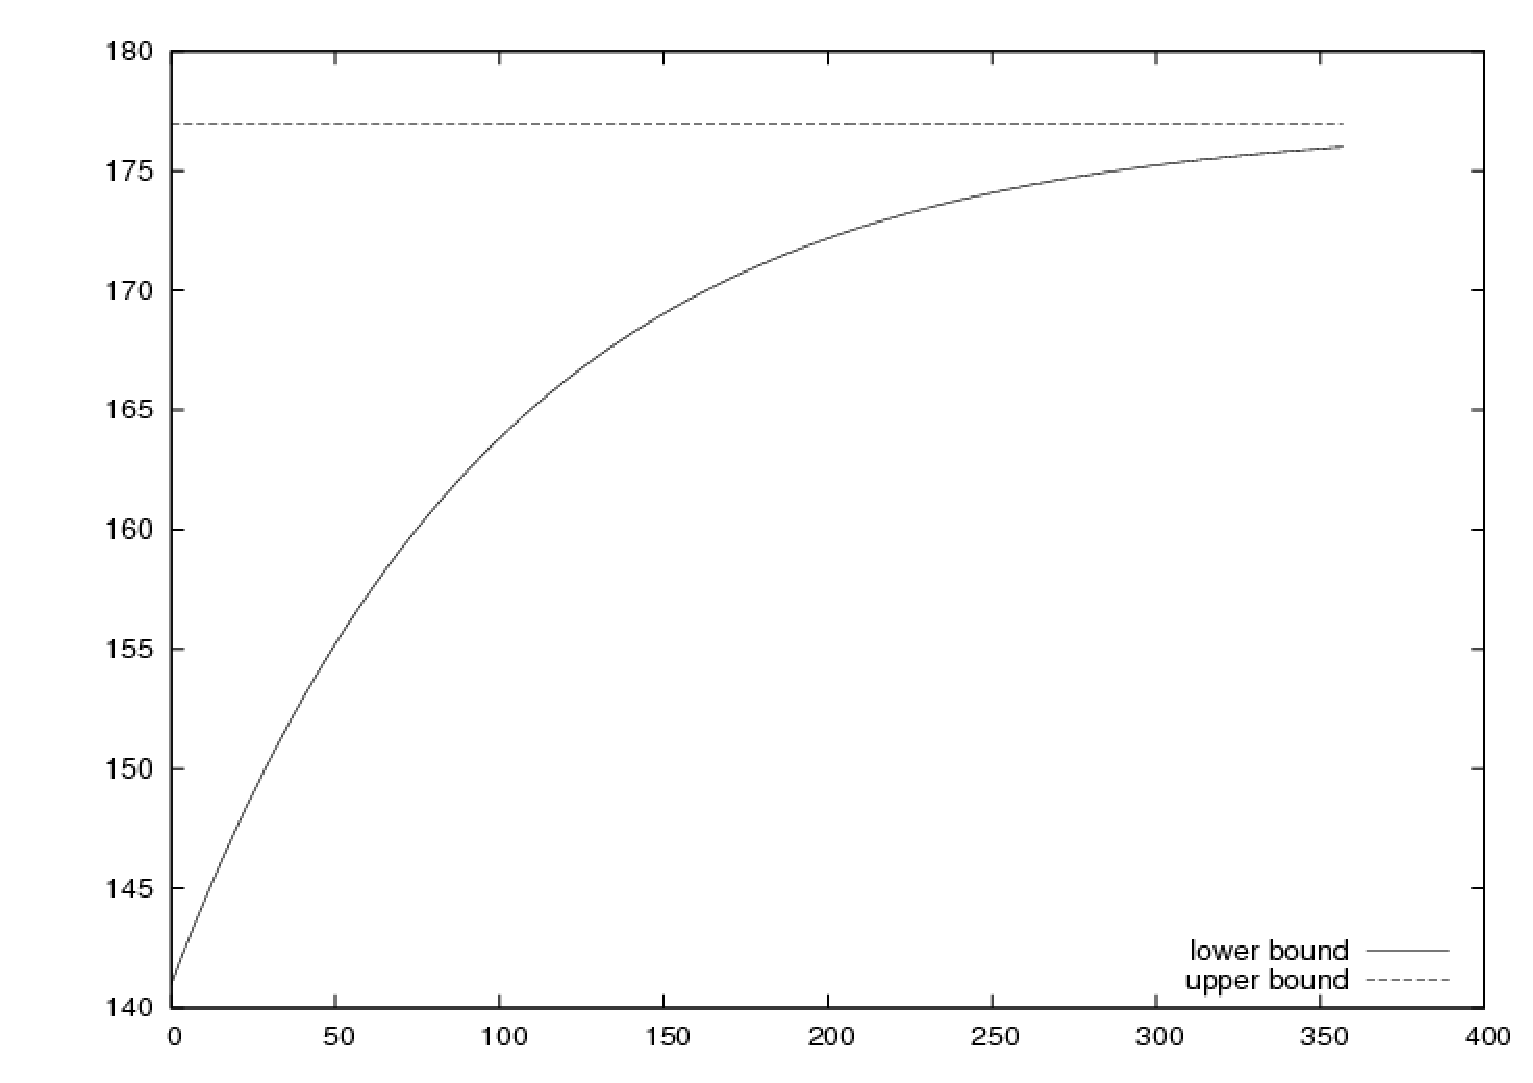
\includegraphics[scale=0.5]{eps/graph_rl1}
  \caption[Gr�fico mostrando a altera��o dos limitantes para a inst�ncia v60\_d30.]{Gr�fico 
  mostrando a altera��o dos limitantes para a inst�ncia v60\_d30 usando a relaxa��o \rl{1} 
  e o arquivo de par�metros do m�todo do subgradiente param3.}
  \label{fig:fig1}
\end{figure}

\newpage{}

\begin{figure}[!htb]
  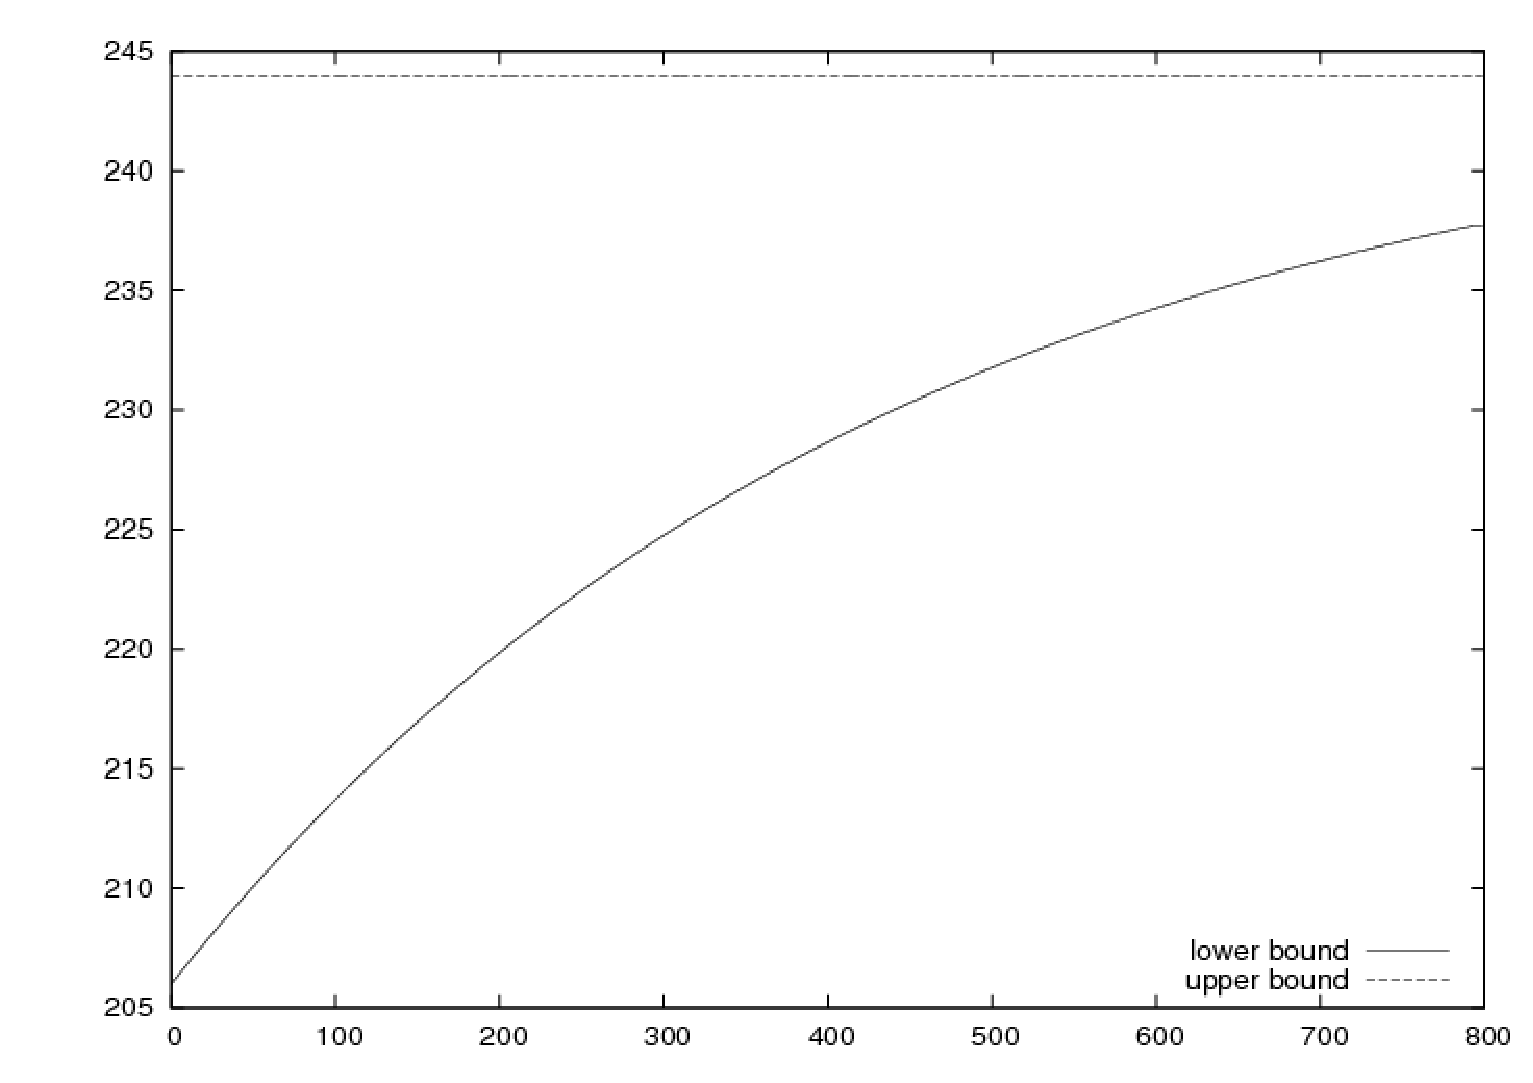
\includegraphics[scale=0.5]{eps/graph_rl2}
  \caption[Gr�fico mostrando a altera��o dos limitantes para a inst�ncia v100\_d5.]{Gr�fico 
  mostrando a altera��o dos limitantes para a inst�ncia v100\_d5 usando a relaxa��o \rl{2} 
  e o arquivo de par�metros do m�todo do subgradiente param3.}
  \label{fig:fig1}
\end{figure}




%\newpage{}
%
%\begin{figure}[htb]
%  \includegraphics[scale=0.5]{graf2}
%  \caption[Gr�fico mostrando a altera��o dos limitantes para a inst�ncia dcmst500\_3.]{Gr�fico mostrando a altera��o dos limitantes para a inst�ncia dcmst500\_3.}
%  \label{fig:fig2}
%\end{figure}
%
%\begin{figure}[htb]
%  \includegraphics[scale=0.5]{graf3}
%  \caption[Gr�fico mostrando a altera��o dos limitantes para a inst�ncia R123\_dcmst200\_3.]{Gr�fico mostrando a altera��o dos limitantes para a inst�ncia R123\_dcmst200\_3.}
%  \label{fig:fig3}
%\end{figure}
%
%\pagebreak{}
%\begin{figure}[htb]
%\centering
%  \includegraphics[scale=0.4]{graph}
%  \caption[Plotagem dos dados obtidos.]{Plotagem dos dados obtidos no experimento.}
%  \label{fig:resultado}
%\end{figure}

\bibliographystyle{plain}
\bibliography{ra046874}

% Fim
\label{fimdoc}
\end{document}
